
\section{Potentialausgleich}
\label{section:blitzschutz}
\begin{frame}%STARTCONTENT

\frametitle{Potentialausgleich und Erdung}
\begin{itemize}
  \item Durch \emph{Potentialausgleich} wird eine gefährliche Berührungsspannung zwischen den Geräten vermieden
  \item Mittels \emph{Erdung} werden unerwünschte elektrische Ströme vom Gehäuse in die Erde abgeleitet
  \end{itemize}
\end{frame}

\begin{frame}
\begin{columns}
    \begin{column}{0.48\textwidth}
    \begin{itemize}
  \item Geräte mittels kurzer Leitungen zusammenführen
  \item Mit Haupterdungsschiene des Gebäudes verbinden
  \item VDE 0855-300 für Erdung von Funkanlagen
  \end{itemize}

    \end{column}
   \begin{column}{0.48\textwidth}
       
\begin{figure}
    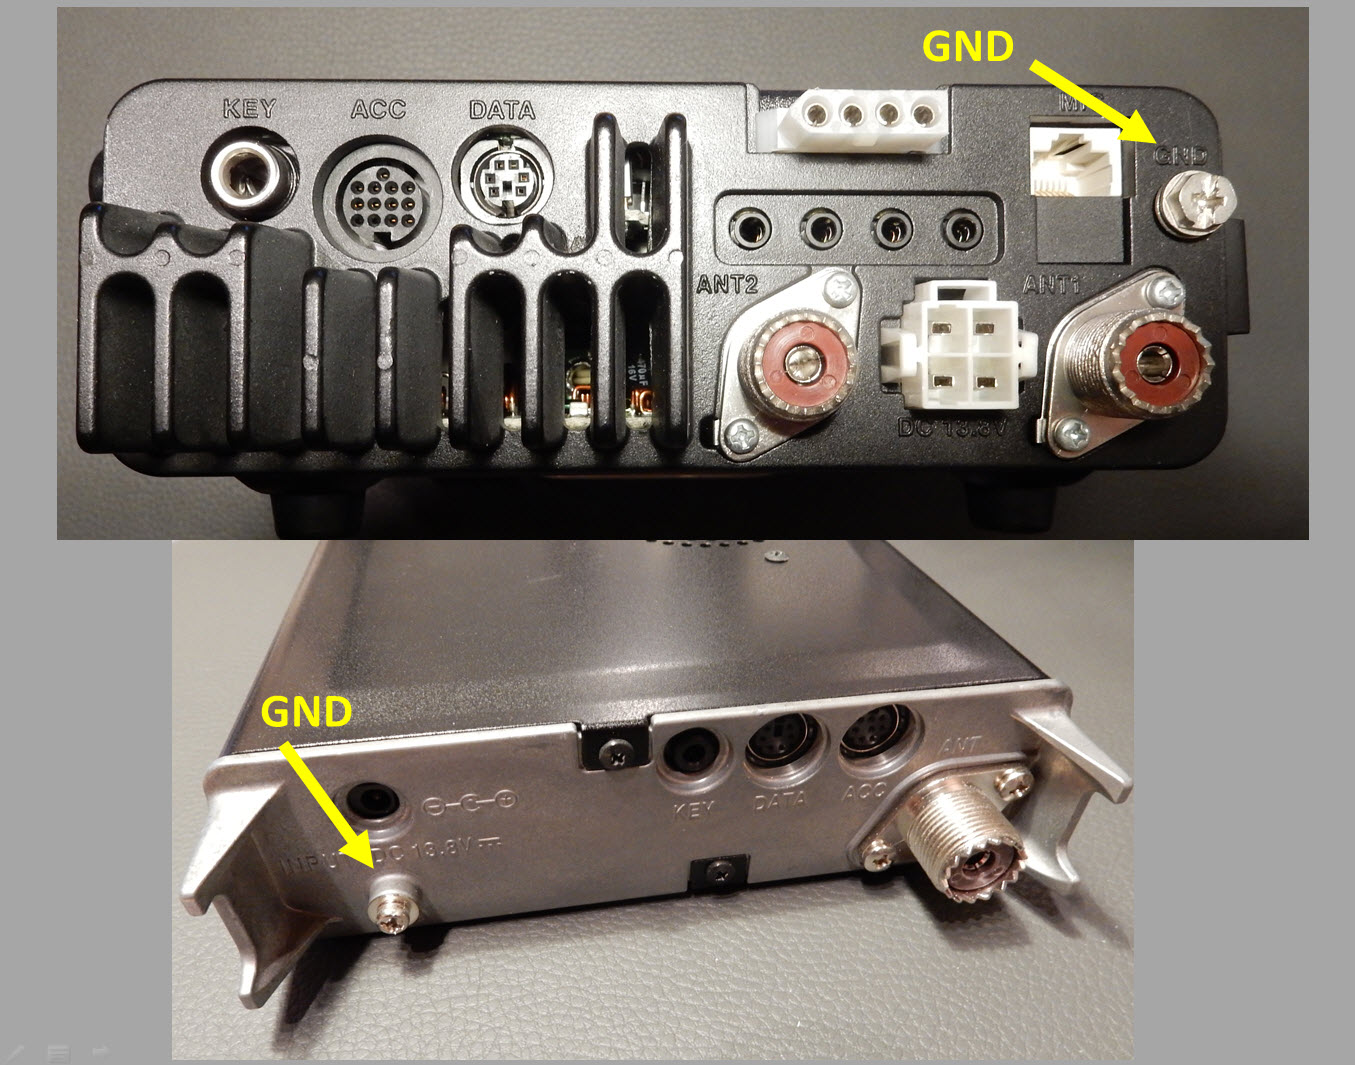
\includegraphics[width=0.85\textwidth]{foto/81}
    \caption{\scriptsize Schraubanschluss Ground (GND) am TRX}
    \label{n_Schraubanschluss_GND}
\end{figure}

   \end{column}
\end{columns}

\end{frame}

\begin{frame}
\frametitle{Achtung}
Der Anschluss von Potentialausgleich und Erdung sollte nur vorgenommen werden, wenn man genau weiß, was man tut. Im Zweifel sollte man sich von einem erfahreneren Funkamateur oder einer Elektrofachkraft helfen lassen.

\end{frame}

\begin{frame}
\only<1>{
\begin{QQuestion}{VE604}{Unter welchen Bedingungen ist die Norm VDE~0855-300 für den Potentialausgleich und die Erdung von Funkanlagen bzw. die Normenreihe VDE~0185-305 zum Blitzschutz heranzuziehen?}{Die Norm VDE~0855-300 gilt für Gebäude, auf denen Antennen errichtet sind. Drahtantennen und freistehende Antennenmasten sind davon ausgenommen.}
{Beide Normen sind dann anzuwenden, wenn Gebäude von Blitzen getroffen werden können.}
{Wenn die Antennenanlage weit genug vom Gebäude entfernt ist, muss die Normreihe VDE~0185-305 nicht angewendet werden.}
{Die Norm VDE~0855-300 gilt für alle Amateurfunk-Sendeanlagen. Die Normenreihe VDE~0185-305 gilt nur für Gebäude mit Blitzschutzsystem.}
\end{QQuestion}

}
\only<2>{
\begin{QQuestion}{VE604}{Unter welchen Bedingungen ist die Norm VDE~0855-300 für den Potentialausgleich und die Erdung von Funkanlagen bzw. die Normenreihe VDE~0185-305 zum Blitzschutz heranzuziehen?}{Die Norm VDE~0855-300 gilt für Gebäude, auf denen Antennen errichtet sind. Drahtantennen und freistehende Antennenmasten sind davon ausgenommen.}
{Beide Normen sind dann anzuwenden, wenn Gebäude von Blitzen getroffen werden können.}
{Wenn die Antennenanlage weit genug vom Gebäude entfernt ist, muss die Normreihe VDE~0185-305 nicht angewendet werden.}
{\textbf{\textcolor{DARCgreen}{Die Norm VDE~0855-300 gilt für alle Amateurfunk-Sendeanlagen. Die Normenreihe VDE~0185-305 gilt nur für Gebäude mit Blitzschutzsystem.}}}
\end{QQuestion}

}
\end{frame}%ENDCONTENT
